\section{Modeling Path Planning as a MILP problem}
This section covers how a trajectory planning problem can be represented as a mixed integer linear program. The problem representation is based on the work by Schouwenaars et al. \cite{Schouwenaars2001}.
\subsection{Overview of MILP}
\label{subsec:previous}
Mixed integer linear programming is and extension of linear programming. In a linear programming problem, there is a single (linear) target function which needs to be minimized or maximized. A problem typically also contains a number linear inequalities which constrain the values of the variables in the objective function. When some (or all) of the variables are integers, the problem is a mixed integer problem. \\
More complex mathematical relations can be modeled by combining multiple constraints. Some of those relations, like logical operators or the absolute value function, can only be expressed when integer variables are allowed \cite{Mitra1994}.

\subsection{Time and vehicle state}
\label{section:modeling}

The trajectory planning problem can be represented with a finite amount discrete time steps with a set of state variables for each epoch. The amount of time steps determines the maximum amount of time the vehicle has in solution space to reach its goal. The actual movement of the vehicle is modeled by calculating the acceleration, velocity and position at each time step based on the state variables from the previous time step. There are $N + 1$ time steps, with a fixed amount of time $\Delta t$ between them.
\begin{equation}
\label{eq:p-start}
\boldsymbol{p}_0 = \boldsymbol{p}_{start}
\end{equation}
\begin{equation}
\label{eq:p-rest}
\boldsymbol{p}_{n+1} = \boldsymbol{p}_{n} + \Delta t * \boldsymbol{v}_{n}  \quad 0 \leq n < N
\end{equation}

Equation \ref{eq:p-start} and \ref{eq:p-rest} model the position of the vehicle at each time step. For each time step $t$, the position in the next time step $p_{n+1}$ is determined by the current position $p_n$, the current velocity $v_n$ and the duration of the time step $\Delta t$. Velocity, acceleration and other derivatives are represented the same way. How many derivatives need to be modeled will vary depending on the specific use case.

\subsection{Objective function}
The objective is to minimize the time before a goal position is reached.

\begin{equation}
\label{eq:goal-fun}
minimize \quad N - \mathlarger{\sum}_{n=0}^{n \leq N} done_n
\end{equation}

Equation \ref{eq:goal-fun} shows the objective function. Reaching the goal causes a state transition from not being done to being done. This is represented as the value of $done_n$, which is a binary variable (which is an integer variable which can only be 0 or 1). When $done_n$ is true (equal to $1$), the vehicle has reached its goal on or before time step $n$.

\begin{equation}
\label{eq:fin-start}
done_0 = 0
\end{equation}
\begin{equation}
\label{eq:fin-end}
done_{N} = 1
\end{equation}
\begin{equation}
\label{eq:fin-rest}
done_{n+1} = done_n \vee cdone_{n+1},  \quad 0 \leq n < N
\end{equation}

Equation \ref{eq:fin-start} initializes $done_0$ to be false, ensuring that the initial state is not finished. Equation \ref{eq:fin-end} forces the state in the last time step to be finished. This means that the vehicle must reach its goal eventually for the problem to be considered solved. \\
Lamport's \cite{Lamport1989} state transition axiom method was used to model state transitions. In equation \ref{eq:fin-rest}, the state will be done at time step $n+1$ if the state is done at time step $n$ or if there is a state transition from not done to done at time step $n + 1$, represented by $cdone_{n+1}$.

\begin{equation}
\label{eq:cfin}
cdone_n =  cdone_{p,t} \wedge \neg done_n\quad 0 \leq n \leq N
\end{equation}

 $cdone_n$ in Equation \ref{eq:cfin} is true at time step $n$ if the goal position requirement $cdone_{p,n}$ is true and the done state has not already been reached ( $ \neg done_n$ ). Additional constraints on the state transition, like a maximum velocity, can be added here.

\begin{equation}
\label{eq:cfin-p}
cdone_{p,n} =  \mathlarger{\mathlarger{\bigwedge_{i = 0}^{i < Dim(\boldsymbol{p}_n)}}} |p_{n,i} - p_{goal, i}| < \epsilon_{p},  \quad 0 \leq n \leq N
\end{equation}

The goal position requirement is represented by $cdone_{p,n}$ and is satisfied when $cdone_{p,n} = 1$. The coordinate in dimension $i$ of the position vector $\boldsymbol{p}_n$, is $p_{n,i}$. The goal position coordinate in that dimension is $p_{goal, i}$. If the difference between those values is smaller than some value $\epsilon_p$ in every dimension at time step $n$,  $cdone_{p,n} = 1$.

\subsection{Vehicle state limits}
\begin{figure}
    \centering
        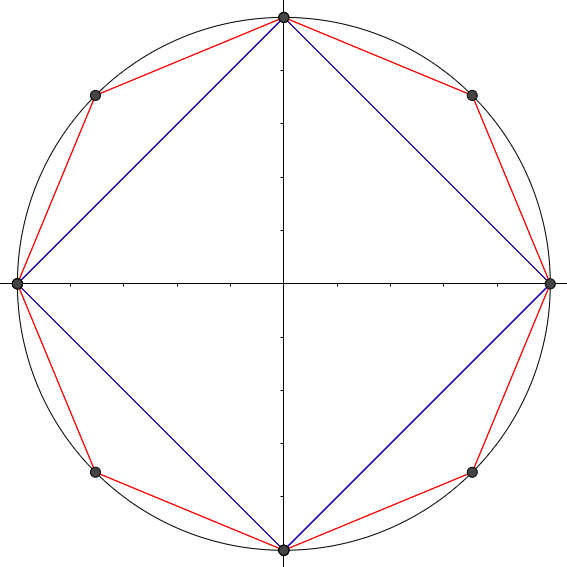
\includegraphics[width=0.6\columnwidth]{img/circlelinear}
    \caption{If the velocity is limited to a finite value, the velocity vector must lie within the circle centered on the origin with the radius equal to that value. This is represented by the black circle. This circle cannot be approximated in MILP, but it can be approximated using several linear constraints. The blue square shows the approximation using 4 linear constraints. The red polygon uses 8 linear constraints. As more constraints are used, the approximation gets closer and closer to the circle. }\label{fig:circlelinear}
\end{figure}
Vehicles have a maximum velocity. Calculating the velocity of the vehicle means calculating the 2-norm of the velocity vector. This is not possible using only linear equations. However, the maximum velocity can be approximated to an arbitrary degree using multiple linear constraints. For simplicity we will cover the 2D case, although this can easily be extended to 3D as well. With $x_i$ and $y_i$ the $N_{points}$ vertices of the approximating polygon listed in counter-clockwise order, the velocity can be limited to $v_{max}$ with Equation \ref{eq:vmax}. Figure \ref{fig:circlelinear} shows a visual representation of these constraints.
%\begin{equation}
%\label{eq:}
%\theta = \dfrac{2\pi}{N_{points}}
%\end{equation}
%\begin{equation}
%\label{eq:}
%x_i  = v_{max} * cos( \theta * i)
%\end{equation}
%\begin{equation}
%\label{eq:}
%y_i  = v_{max} * sin( \theta * i)
%\end{equation}
\begin{equation}
\label{eq:lin-a}
a_i = \dfrac{y_{i} - y_{i-1}}{x_{i} - x_{i-1}} \quad 0 \leq i < N_{points}
\end{equation}
\begin{equation}
\label{eq:lin-b}
b_i = y_{i} - a_i x_i  \quad 0 \leq i < N_{points}
\end{equation}
\begin{equation}
\label{eq:vmax}
v_{n, 1} \leq a_i v_{n,0} + b_i  \quad 0 \leq i < N_{points}, ~ 0 \leq n \leq N
\end{equation}


The acceleration and other vector properties of the vehicle can be limited in the same way. This method can also be applied to keep the vehicle's position inside a convex polygon.
\subsection{Obstacle avoidance}

\begin{figure}[!t]
    \centering
    \subfloat{
        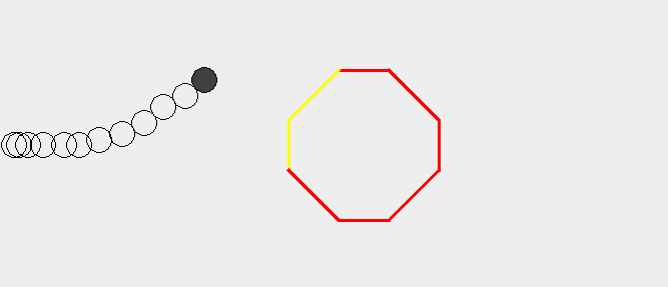
\includegraphics[width=0.8\columnwidth]{img/obs1}
    }
    \hfil
     \subfloat{
        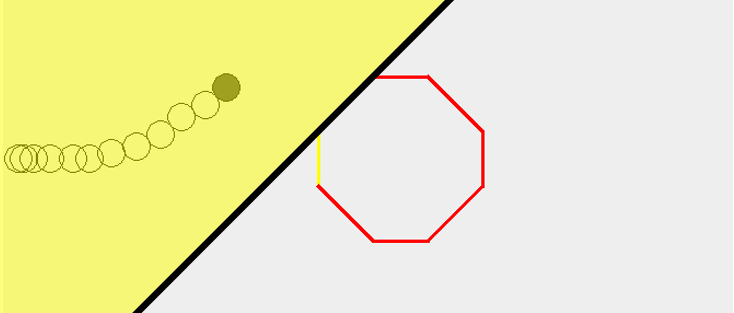
\includegraphics[width=0.8\columnwidth]{img/obs2}
     }
     \hfil
     \subfloat{
        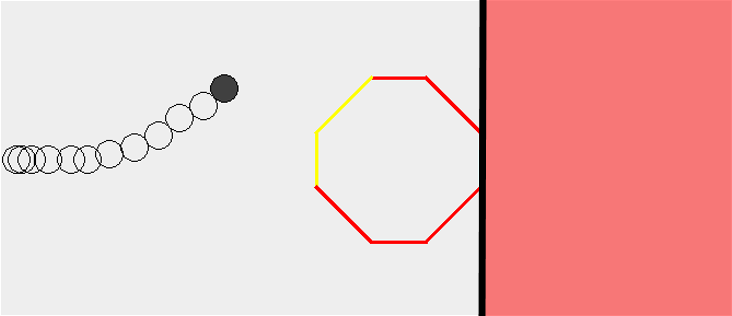
\includegraphics[width=0.8\columnwidth]{img/obs3}
     }
    \caption{A visual representation of how obstacle avoidance works. The top image shows the vehicle's current position as the filled circle, with its trajectory in previous time steps as hollow circles. The color of the edges of the obstacle represent whether or not the vehicle is in the safe zone for that edge. An edge is yellow if the vehicle is in the safe zone, and red otherwise. The middle image shows the safe zone defined by a yellow edge in yellow. Note how the vehicle is on one side of the black line and the obstacle is entirely on the other side. The bottom image shows an edge for which the vehicle is not in the safe zone (represented in red this time). As long as the vehicle is in the safe zone of at least one edge, it cannot collide with the obstacle.}\label{fig:obs}
\end{figure}
The most challenging part of the problem is modeling obstacles. Any obstacle between the vehicle and its goal will inherently make the search space non-convex. Because of this, integer variables are needed to model obstacles. For each edge of the polygon obstacle, the line through that edge is constructed. If the obstacle is convex, the obstacle will be entirely on one side of that line. This means that the other side can be considered a safe area. However, the vehicle cannot be in the safe area of all edges at the same time, so a mechanism is needed to turn off these constraints when needed. As long as the vehicle is in the safe area of at least one edge, it cannot collide.  Figure \ref{fig:obs} demonstrates this visually. \\
The most common way to turn off individual constraints is using the ``Big M'' method, like Schouwenaars et al. \cite{Schouwenaars2001} used in their work. However CPLEX supports a better method called ``indicator constraints''. Just like with the Big M method, it requires one boolean variable per edge. If the variable is true, the corresponding constraint is ignored. As long as at least one of those variables if false, a collision cannot happen. We will call these slack variables. For every convex obstacle $o$ with vertices $x_{o,i}$ and $y_{o,i}$ with $a_{o,i}$ and $b_{o,i}$ calculated as in equations \ref{eq:lin-a} and \ref{eq:lin-b}:
\begin{equation*}
dx_{o,i} = x_{o,i} - x_{o,i-1}, \quad dy_{o,i} = y_{o,i} - y_{o,i-1}
\end{equation*}
\begin{equation}
\label{eq:obs}
slack_{o,i,t} \Rightarrow \\
\begin{cases}
b_i + offset_{o,i} \leq p_{t,1} - a_i p_{t,0} & dx_{o,i} < 0 \\
b_i - offset_{o,i}  \geq p_{t,1} - a_i p_{t,0} & dx_{o,i} > 0 \\
%x_{o,i} + buf_{o,i}  \leq p_{t,0} & dx_{o,i} = 0, dy_{o,i} > 0 \\
%x_{o,i} - buf_{o,i}  \geq p_{t,0} & dx_{o,i} = 0, dy_{o,i} < 0 \\
\parbox[t]{.4\columnwidth}{ \vspace{-0.25\baselineskip} $x_{o,i} + offset_{o,i}  \leq p_{t,0}$ } & \parbox[t]{.25\columnwidth}{ $dx_{o,i} = 0$, \\ $dy_{o,i} > 0$ } \\
\parbox[t]{.4\columnwidth}{ \vspace{-0.25\baselineskip} $x_{o,i} - offset_{o,i}  \geq p_{t,0}$ } & \parbox[t]{.25\columnwidth}{ $dx_{o,i} = 0$, \\ $dy_{o,i} < 0$ } \\

\end{cases}
\end{equation}
\begin{equation}
\neg \mathlarger{\mathlarger{\bigwedge_{i}}} slack_{o,i,n} \quad 0 \leq n \leq N
\end{equation}

The occurrences of $offset_{o,i}$ in equation \ref{eq:obs} are necessary because the vehicle is not a point. The position variables represent the position of the center of mass of the vehicle. With the shape of the vehicle approximated as a circle of radius $S$ and $\alpha_{o,i}$ the angle perpendicular to edge $i$ of obstacle $o$:
\begin{equation}
\alpha_{o,i} = tan^{-1}( -1 / a_{o,i})
\end{equation}
\begin{equation}
offset_{o,i} = |\dfrac{S}{sin(\alpha_{o,i})}|
\end{equation}

Modeling obstacles this way is problematic because an integer variable is needed for every edge of every obstacle, for every time step. Each integer variable makes the solution space less convex, increasing the worst case execution time exponentially \cite{DBLP:conf/coco/Karp72}.